\scanpage{125}
% archive foliation: 124
que $A\cup[0,1]$ soit un $1$-complexe.

Pour que de plus les $A_X$ \deleted{\unsure{soient définis}}
sur les $X$ de nouvelles structures de
Cartes (i.e. $X\setminus A_X$ a comp. conn. $\simeq$ disques)
il f. et s. que a) $A$ soit connexe
\deleted{\unsure{Ou si $A$ ne l'est plus}}\par
\deleted{b) $A$ contienne deux des pts $0,1,\infty$ (\unsure{ou au moins}}\par
\deleted{\unsure{s'il laisse plus des pts $0,1,\infty$ qui ne $\in A$})}\par
\deleted{\unsure{ou bien}}\par
\inserted{i.e. définisse une carte sur $S^1$}

b) \deleted{\unsure{À une face}} \unsure{aucune des} \deleted{\unsure{deux}} \unsure{dites cartes}
ne peut contenir au plus qu'un seul
des pts $0,1,\infty$.

Supposons cette condition satisfaite. Choisissons
des sommets de $A$, \deleted{\unsure{et}} des centres des
faces, des milieux d'arêtes, de façon
à satisfaire à $2$ conditions:

$1^\circ)$ Si \deleted{\unsure{un}} des pts $0,1,\infty$ est dans une
face ouverte, on le choisit comme
centre de la dite [il n'y a pas de conflit\ldots]

$2^\circ)$ Sinon (i.e. \deleted{\unsure{s'il est}} $s\in A$] on choisit $s$
comme un sommet de $A$, \deleted{\unsure{à}} à l'exception
du seul cas qui suit:
\margin{\unsure{on n'est pas obligé de faire}, \unsure{i.e.} \unsure{choisir tous les sommets topolog. des $A_X$}\ldots}

$3^\circ)$ Si $s=1\in A$, et si $s$ est \deleted{un} \inserted{un} pt
d'ordre $1$ de $A$\par
i.e. un bout
\figure{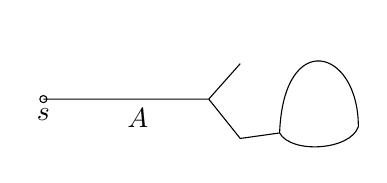
\begin{tikzpicture}[x=1cm,y=1cm]
\draw (0,0)--(2.1,0)--(2.5,.45);
\draw (2.1,0)--(2.5,-.5)--(3,-.43) .. controls (3.05,.9) and (4,.65) .. (4,-.35) .. controls (3.9,-.65) and (3.15,-.7) .. (3,-.43);
\draw (0,0) circle (.045);\node[below] at (0,0) {$s$};\node[below] at (1.2,0) {$A$};
\end{tikzpicture}}
